\documentclass{article}
\usepackage[spanish]{babel} % Agregamos la ortografía española
\usepackage[utf8]{inputenc} % Agregamos las tildes
\usepackage{amsmath} % Sin este no podría usar ciertos entornos como el de ecuación
\usepackage{amssymb} % Sin este no puedo usar algunos símbolos matemáticos
\newtheorem{teorema}{Teorema}
\newtheorem{colorario}{Colorario}
\usepackage{color}
\usepackage{graphicx} %Para poder introducir gráficos
\usepackage{float}
\renewcommand{\listtablename}{Índice de tablas}
\renewcommand{\tablename}{Tabla}



\begin{document}

\tableofcontents
\title{Introducción a LaTeX}
\author{Pedro Estévez}
\maketitle

\begin{abstract}
En este artículo daremos los primeros ejemplos de la creación de textos con LaTeX.
\end{abstract}

\section{Introducción}
\subsection{Formato de texto}
\subsubsection{Normas de ortografía} % Ya no puedes más, ahora tienes que usar paragraph.
\paragraph{Ejemplos.}

Ejemplos de letras griegas $\alpha$, $\beta$. 
Para crear una fórmula que esté separada del resto del texto, he de poner dos símbolos de dolar.
 $$(\alpha+\beta)^2=\alpha^2+\beta^2+2\alpha\beta$$
Para agregar la ortografía española, así como las tildes, he de inicializar dos paquetes.\bigskip
% Si queremos poner una tilde pero aislada, por ejemplo en un documento que no está escrito en español, usamos f\'ormula

Otro ejemplo. La integral de fourier tiene período $2\pi/T$.
Matemáticas más complejas: 
Sea $\{\tilde{\gamma}_{ij}\}_{0\leq i+j \leq 2n}$ una \textbf{aplicación} inyectiva sobre el {\bf espacio} cambia el tipo de \emph{escritura}.\bigskip

Una fórmula conocida es $$\sum_{k=1}^n k=\frac{n(n+1)}{2}$$

Veamos un ejemplo más complejo de fracciones 
$$\frac{\frac{a}{x-y}+\frac{b}{x+y}}{1+\frac{a-b}{a+b}}$$

Para construir matrices 
$$\begin{pmatrix}
1&5\\
-2&3
\end{pmatrix}$$ % La p es de paréntesis, si la quitas, no los pone, tendrías que hacer lo siguiente

$$\left(\begin{matrix}
1&5&-3\\
2&-8&3\\
6&-7&1
\end{matrix}\right)$$

$$
\psi(x)=\begin{cases}
Ae^{ikx}+Be^{-ikx}, &\mbox{si $x=0$}\\
De^{ikx}, &\mbox{si $x\neq 0$}
\end{cases}
$$

Ahora una parte muy importante, el entorno ecuación, que me numerará automáticamente las fórmulas.
\begin{equation}\label{eq1}
\varphi(x,z)=z-\gamma_ {10} x- \sum_ {m+n\geq 2} \gamma_{mn} x^m z^n
\end{equation}

Podemos citar una de las fórmulas de forma que si luego cambiamos algún orden, éste se cambia automáticamente. Por ejemplo \eqref{eq1}.\bigskip

Con el entorno eqnarray puedo poner sistemas, ya que si pusiera las ecuaciones seguidas se notaría un espacio demasiado grande.
\begin{eqnarray}
x+y+z=2\nonumber\\
x-y-z=1\label{eq2}\\
x-y+z=3\nonumber
\end{eqnarray}

Y ahora podemos llamar a la ecuación como si fuera el sistema entero. Por ejemplo \eqref{eq2}
\\ [4mm]
\indent
Por último, hoy veremos como poner teoremas, lemas, colorarios etc. Tenemos que inicializarlo.
\begin{teorema}
Si tenemos una función f(x) contínua y derivable...
\end{teorema}

\begin{teorema}
Si tenemos una función f(x) contínua y derivable vemos que podemos poner muchos.
\end{teorema}

\begin{colorario}
Lo mismo para otros elementos.
\end{colorario}

Nuevo entorno. La única diferencia entre este entorno y el entorno eqnarray es que éste te numera el sistema entero en vez de cada ecuación.
\begin{equation}
\begin{split}
\frac{d^2y}{dt^2}+\omega^2x=0\\
y(0)=1,\ y'(0)=0 % La barra separa un poco. Si pongo \quad separa más y si uso \qquad más.
\end{split}
\end{equation}

Para poner notas a pie de página.\footnote{Nótese como he creado una nota aquí}\smallskip

Si quiero poner algo con comillas, no es tan fácil como pone comillas``caballero".\copyright\smallskip 

Quedé en primera posición --- Quedé en 1\textsuperscript{a} posición.\smallskip

El Quijote vuajó por ciudad real \textcolor{red}{a caballo}.\smallskip

Veamos ejemplos de cómo hacer listas con LaTeX. Sea $f$ una función que satisface lo siguiente:
\begin{enumerate}
\item $f$ es contínua.
\item $f$ es integrable a trozos.
\begin{itemize}
\item Podemos crear sublistas
\item Esto es muy útil
	\end{itemize}
\item $f$ es nula en un conjuntos de medida positiva.
\end{enumerate}


\begin{itemize}
\item $f$ es contínua.
\item $f$ es integrable a trozos.
\item $f$ es nula en un conjuntos de medida positiva.
\end{itemize}

\begin{description}
\item{a)} $f$ es contínua.
\item{b)} $f$ es integrable a trozos.
\item{c)} $f$ es nula en un conjuntos de medida positiva.
\end{description}

Para introducir figuras, las figuras deben estar en la misma carpeta que todos los archivos de LaTeX
$$
\frac{d^2\psi}{dt^2}+\nabla^2\psi=V(x)\psi
$$
Las órbitas heteroclinas de sus soluciones vienen dadas por la siguiente figura: 
\begin{center}
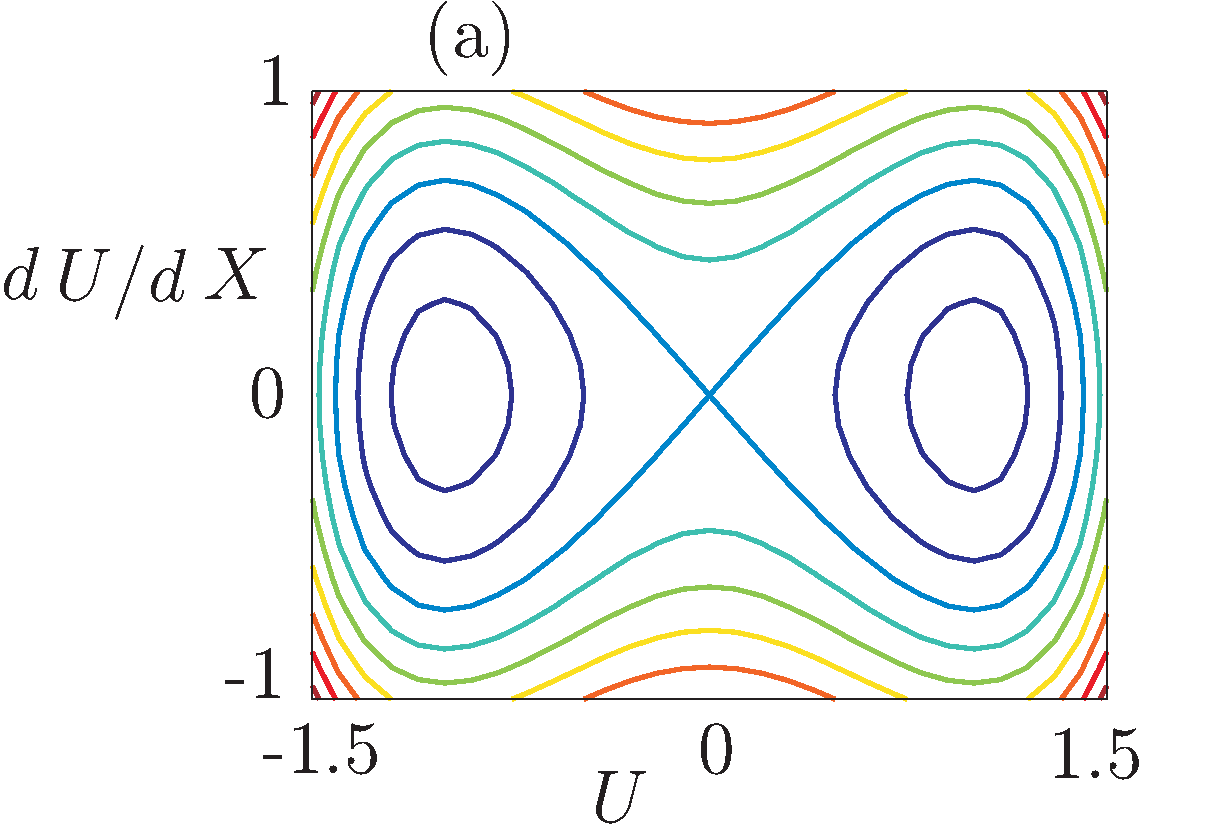
\includegraphics[width=5cm,height=3.5cm]{figura1} % Si pongo solo width, latex me lo sescala perfectamente para mantener las dimensiones.
\end{center}
\begin{center}
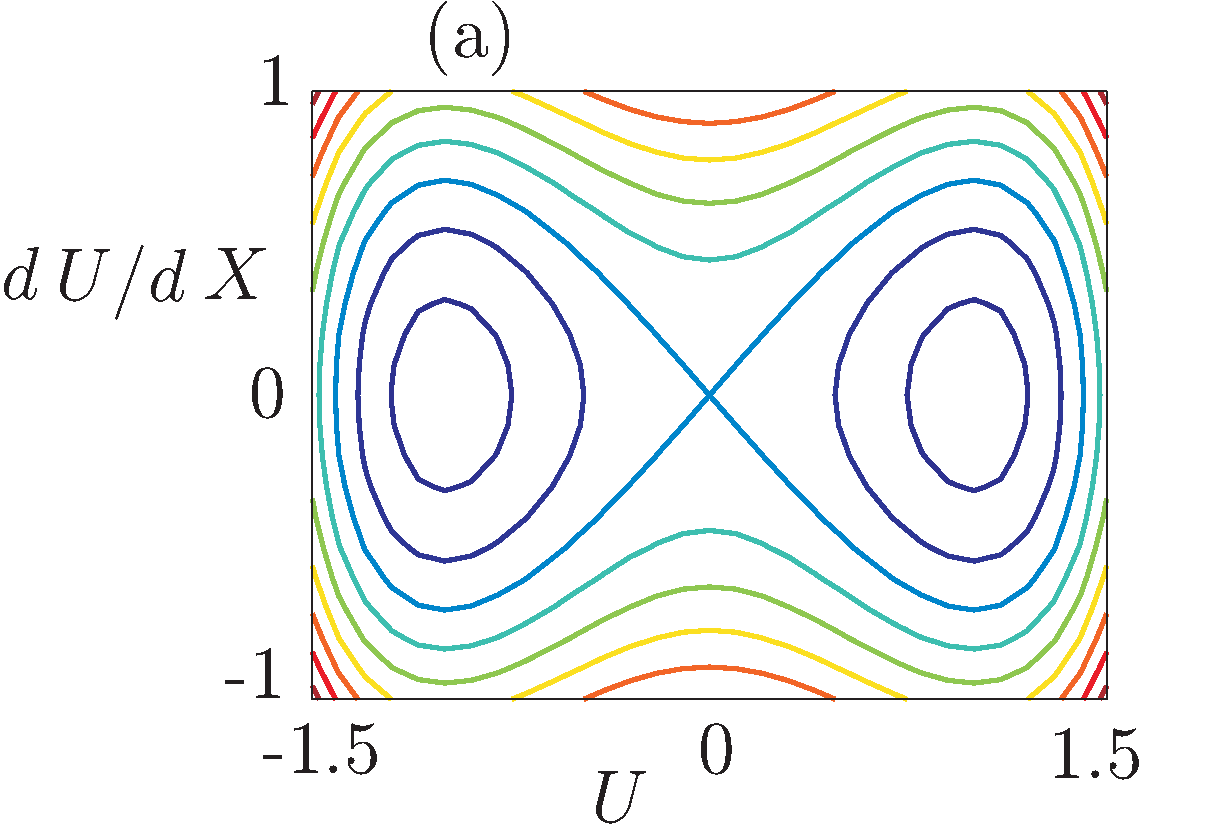
\includegraphics[scale=0.28]{figura1} % Por defecto, 1 es el tamaño original.
\end{center}

Si quiero insertar las imágenes de forma que formen una matriz \smallskip
\begin{figure} % Al ahcer esto convierto las figuras a objetos flotantes (latex decide el mejor sitio para poner la foto), permitiéndome poner pie de foto. Si pongo despues de figure [h] de here, me pondrá la foto en el lugar que yo le digo en vez de en el sitio que mejor considere latex. (Seguir escribiendo)
\begin{center}
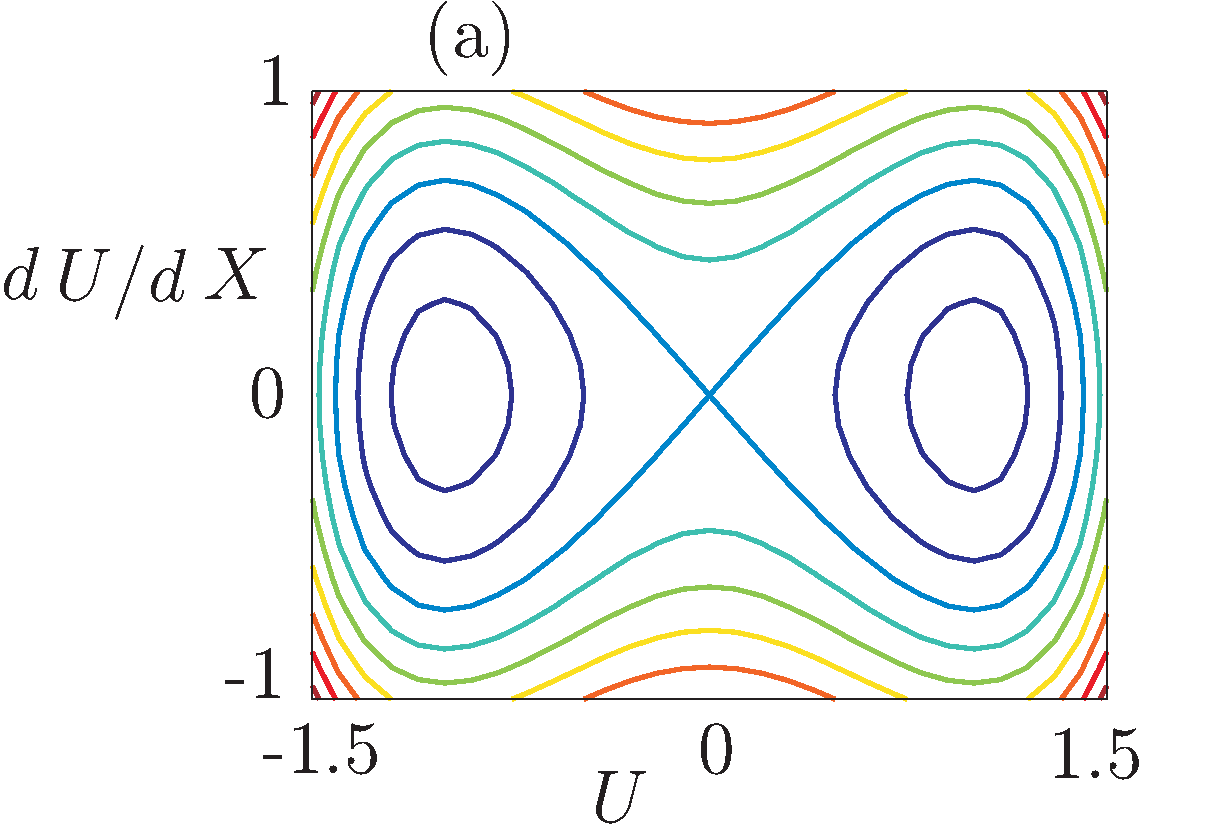
\includegraphics[scale=0.25]{figura1}
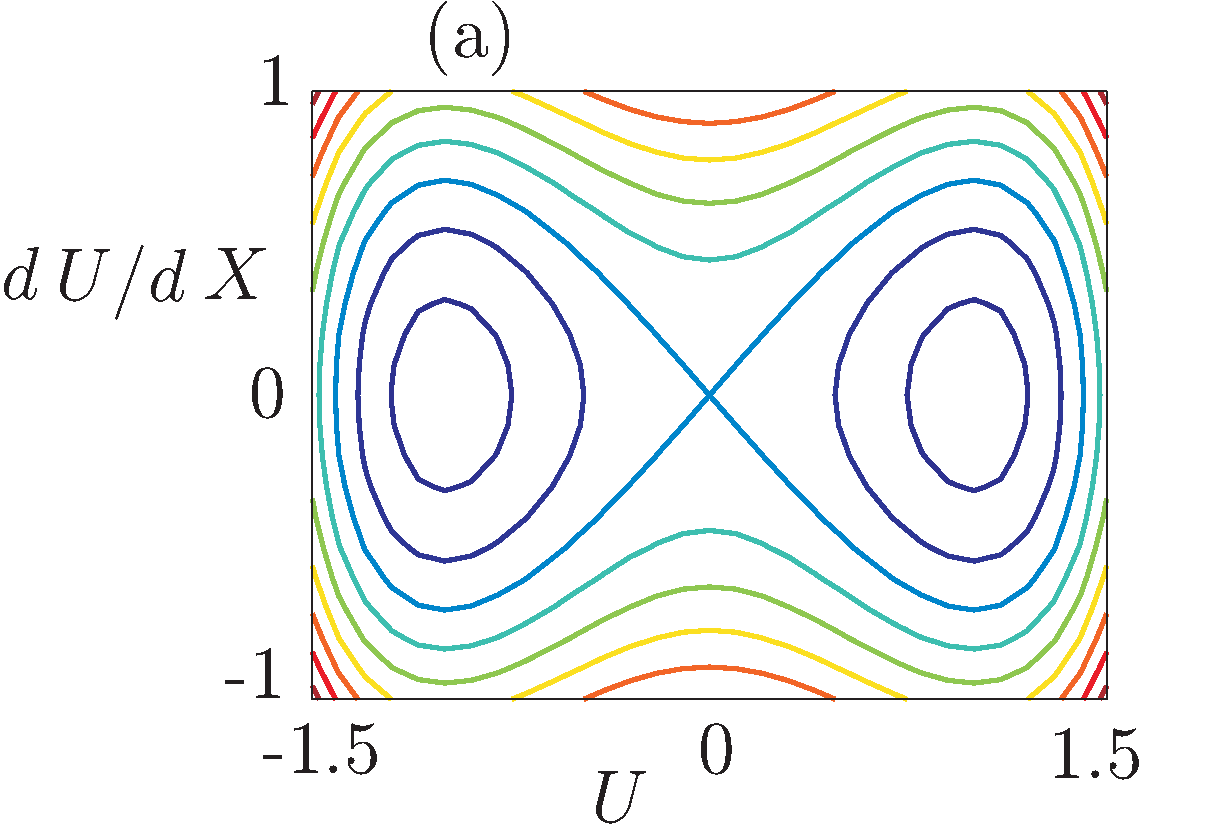
\includegraphics[scale=0.25]{figura1}\\
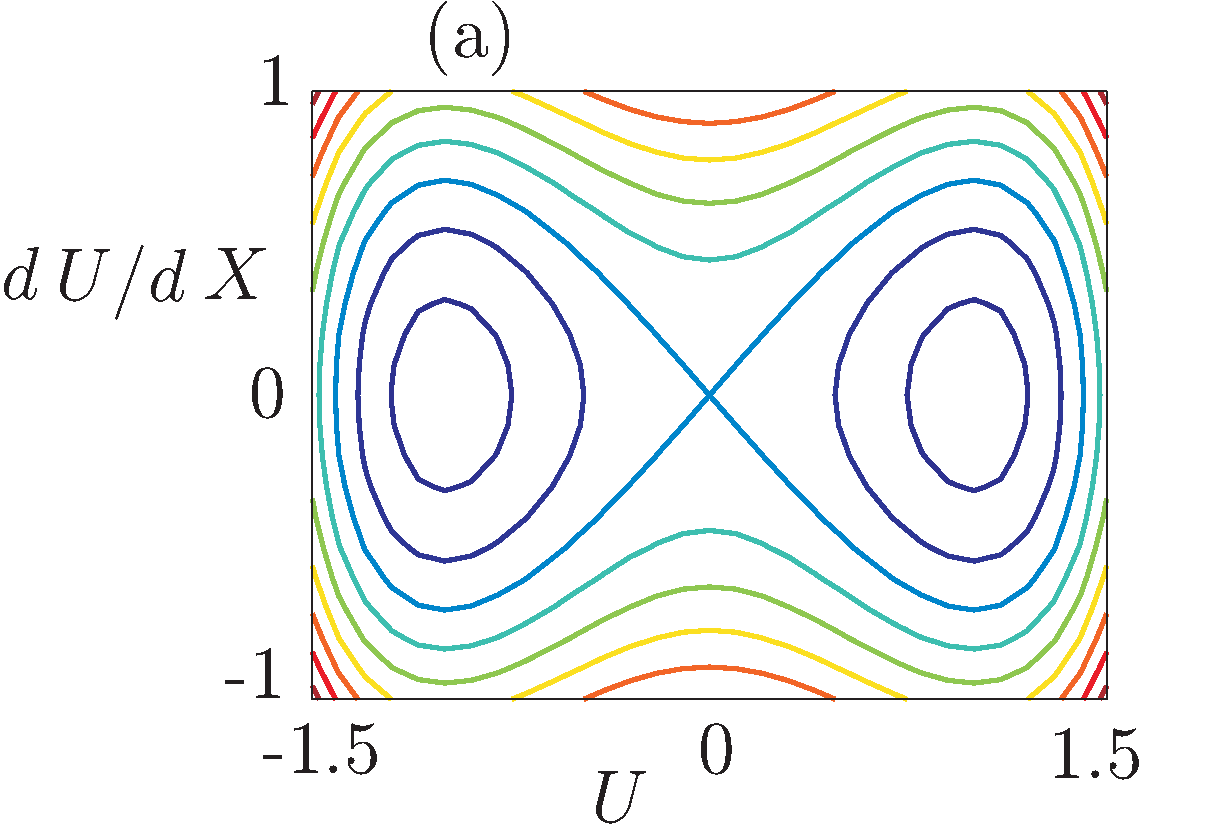
\includegraphics[scale=0.25]{figura1}
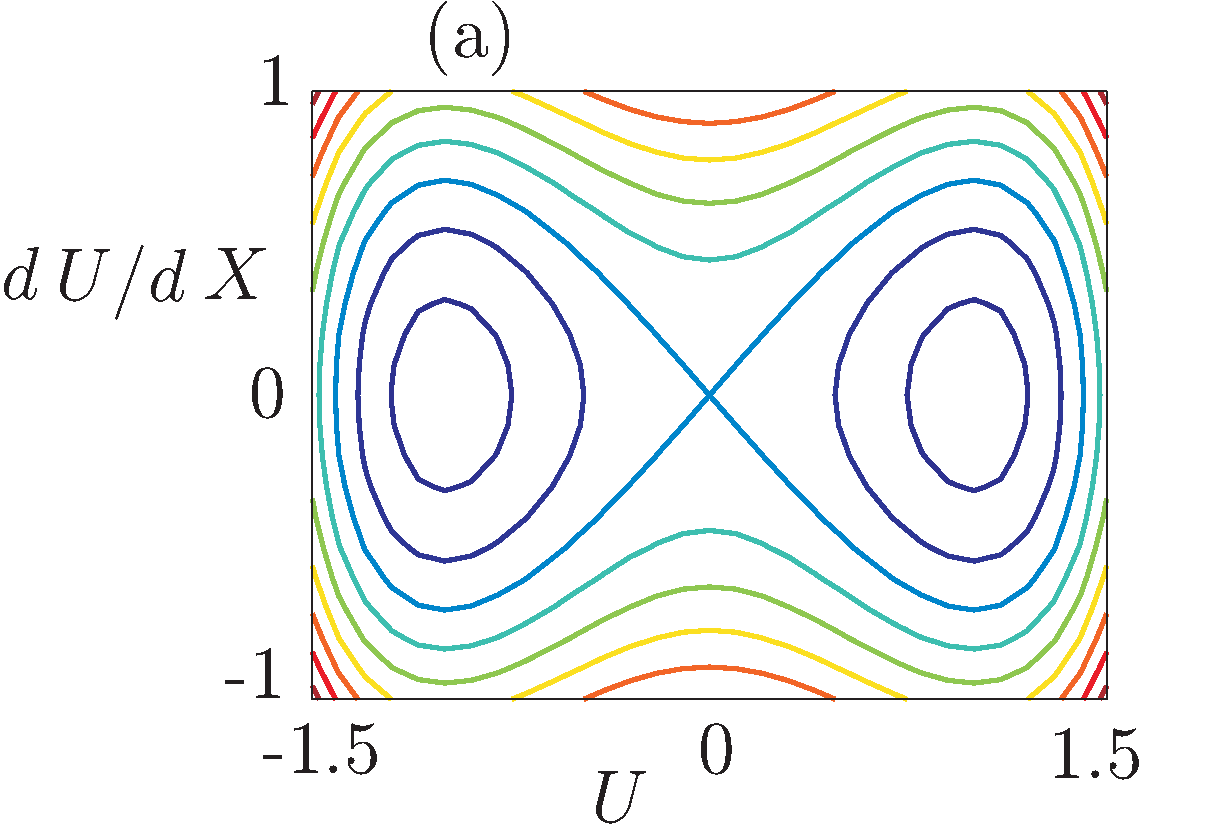
\includegraphics[scale=0.25]{figura1}
\caption{Estas figuras muestran como hacer una disposición en matriz} \label{fig1} % IMPORTANTE	. Hacerlo en el caption, si no me la nombra mal.
\end{center}
\end{figure}

También las podemos llamar del modo habitual, \ref{fig1} \bigskip


Veamos ahora cómo crear tablas
\begin{table}[H] %Para convertir la tabla a objeto flotante y poder ponerle pie de foto
\begin{center}
\begin{tabular}{|c|c|c|} \hline % Para hacer la tabla
\multicolumn{3}{|c|}{Tabla con numeros}\\ \hline
uno&dos&tres\\ \hline \hline
cuatro&cinco&seis\\ \hline
siete&ocho&nueve\\ \hline
diez&once&doce\\ \hline
trece&\multicolumn{2}{|c|}{catorce}\\ \hline
\end{tabular}
\caption{Y así es como se ha ce una tabla}\label{tabla1}
\end{center}
\end{table}

Y, por supuesto, la podemos llamar \ref{tabla1}. Parece ser que funciona













\end{document}